% senior_thesis-proposal.tex
% CMPSC 580, Spring 2016
%
%
% This document provides a sample senior thesis proposal template for use
% by students in Allegheny's CS and Applied Computing programs.
%
%   *******************************************************************
%   * LOOK FOR BLOCK COMMENTS SUCH AS THIS ONE FOR AN EXPLANATION OF  *
%   * THIS DOCUMENT AND HOW TO MODIFY IT FOR YOUR OWN PROPOSAL!       *
%   *                                                                 *
%   * ANY LINE BEGINNING WITH A "%" IS A LATEX COMMENT AND IS IGNORED *
%   * BY THE LATEX PROCESSOR. YOU ARE ENCOURAGED TO COMMENT YOUR OWN  *
%   * LATEX CODE.                                                     *
%   *******************************************************************

%   ********************************************************************
%   * THE FIRST SECTION OF THE LATEX FILE IS THE "PREAMBLE." IT        *
%   * INSTRUCTS LATEX TO IMPORT SPECIAL PACKAGES FOR THINGS LIKE       *
%   * INCLUDING FIGURES, DOUBLE-SPACING, COLORED TEXT, ETC.            *
%   * DEPENDING ON YOUR NEEDS, YOU MAY FIND IT NECESSARY TO USE PACK-  *
%   * AGES THAT ARE NOT INCLUDED IN THIS TEMPLATE. SIMPLY IMITATE THE  *
%   * "\usepackage{...}" COMMANDS SHOWN BELOW.                         *
%   ********************************************************************

%   ********************************************************************
%   * BEGINNING OF PREAMBLE:                                           *
%   ********************************************************************
\documentclass[11pt]{article}

\usepackage[T1]{fontenc}
\usepackage{mathptmx}
\topmargin 0.0in
\setlength{\textwidth} {420pt}
\setlength{\textheight} {620pt} 
\setlength{\oddsidemargin} {20pt}
\setlength{\marginparwidth} {72in}

%   ********************************************************************
%   * Many of the commands below were simply copied over from an older *
%   * version of the proposal template; you can just leave them as     *
%   * they are (or you can delve into the TeX/LaTeX documentation      *
%   * and figure out what they do). Otherwise, jump ahead to the next  *
%   * block of comments, where you will enter title, abstract, etc.    *
%   ********************************************************************

\usepackage{fancyhdr} 
\usepackage{url}
\usepackage{hyperref}
\usepackage{graphicx}
\usepackage{cite}

\usepackage{tikz}
\usetikzlibrary{shapes.geometric, arrows}

% set it so that subsubsections have numbers and they
% are displayed in the TOC (maybe hard to read, might want to disable)

\setcounter{secnumdepth}{3}
\setcounter{tocdepth}{3}

% define widow protection

\def\widow#1{\vskip #1\vbadness10000\penalty-200\vskip-#1}

\clubpenalty=10000  % Don't allow orphans
\widowpenalty=10000 % Don't allow widows

% this should give me the ability to use some math symbols that 
% were available by default in standard latex (i.e. \Box)

\usepackage{latexsym}

% define a little section heading that doesn't go with any number

\def\littlesection#1{
\widow{2cm}
\vskip 0.5cm
\noindent{\bf #1}
\vskip 0.0001cm 
}

\pagestyle{fancyplain}

\newcommand{\tstamp}{\today}   
\renewcommand{\sectionmark}[1]{\markright{#1}}
\lhead[\Section \thesection]            {\fancyplain{}{\rightmark}}
\chead[\fancyplain{}{}]                 {\fancyplain{}{}}
\rhead[\fancyplain{}{\rightmark}]       {\fancyplain{}{\thepage}}
\cfoot[\fancyplain{\thepage}{}]         {\fancyplain{\thepage}{}}

\newlength{\myVSpace}% the height of the box
\setlength{\myVSpace}{1ex}% the default, 
\newcommand\xstrut{\raisebox{-.5\myVSpace}% symmetric behaviour, 
  {\rule{0pt}{\myVSpace}}%
}

% leave things with no spacing extra spacing in the final version of the paper
\renewcommand{\baselinestretch}{1.0}    % must go before the begin of doc

% suppress the use of indentation for a paragraph

\setlength{\parindent}{0.0in}
\setlength{\parskip}{0.1in}

\begin{document}


% handle widows appropriately
\def\widow#1{\vskip #1\vbadness10000\penalty-200\vskip-#1}

% build the title section

\makeatletter

\def\maketitle{%
  %\null
  \thispagestyle{empty}%
  %\vfill
  \begin{center}%\leavevmode
    %\normalfont
    {\Huge \@title\par}%
    %\hrulefill\par
    {\normalsize \@author\par}%
    \vskip .4in
%    {\Large \@date\par}%
  \end{center}%
  %\vfill
  %\null
  %\cleardoublepage

  }

\makeatother

%   ********************************************************************
%   * Here is the first place where you need to begin customizing:     *
%   * Enter you name, the title of your proposal, etc., in the places  *
%   * indicated by the comment "% CHANGE!".                            *
%   ********************************************************************

\vspace*{-1.1in}
\title{Measuring the Digital Footprint \\ \Large A Tool for Understanding the Data Collected from Internet Users}  % CHANGE!

% build the author section
\author{
        Zachary M. Shaffer\\  % CHANGE!
        Department of Computer Science\\
        Allegheny College \\
        {\tt shafferz@allegheny.edu}  \\  % CHANGE!
        \url{http://shafferz.github.io} \\  % CHANGE OR DELETE!
        \vspace*{.1in} \today \\ \vspace*{.1in}
}

\maketitle       % use the default title stuff

% Default "abstract" environment is too small; customize one instead:
\begin{center}
\large\bf Abstract
\vspace{-1em}  % Reduce space between header and the abstract
\end{center}

%   ********************************************************************
%   * Here is the second place where you need to customize:            *
%   * enter your abstract in the "quote" environment:                 *
%   ********************************************************************

\begin{quote}
Every week, hundreds of millions of Americans access the internet for billions of hours. In this time, the user generates a distinct digital footprint that can be used to identify the user's personal information and browsing habits, such as legal names, addresses, phone numbers, entertainment viewing habits, social media accounts, email addresses, and much more. These deeply personal dossiers of information can be linked to a given user with a plurality of tools, cookies, and other unique pieces of identifying information. Since most Americans have concerns about their digital privacy, this thesis proposes a tool that will identify, measure, and present a user with their own digital footprint, and give the user advice on how to reduce the transparency of this information. This tool is being developed on the forefront of an age when digital privacy is a major concern throughout the United States as a topical and poignant subject.
\end{quote}

%\vspace*{-.4in}
\section{Introduction}
\label{sec:introduction}
\vspace*{-.1in}

%   ********************************************************************
%   * Enter the text of your introductory section here.                *
%   ********************************************************************

In 2016, the average American internet user spent about 23.6 hours online each week\cite{digital-future}. As of June 30, 2017, there are over 286 million American internet users. That is a collective 6.7 billion hours spent online in America alone, and America only accounts for 9.8\% of all internet usage worldwide\cite{internet-world-stats}. Keeping track of what any one given individual does online, then, should seem to be fairly difficult. That is not the case, however, as websites are using information given by users who access the internet to build and sell profiles of any given individual user. 

This collection of information on a user, known as the user's digital footprint, can tell a website anything ranging from their location and IPv6 address, to what kinds of videos the user likes to watch online, or even what kind of products they like to purchase. The average user, however, is typically unaware of the kind of information they are providing to these websites. The motivation for the creation of a digital footprint measuring tool comes from the simple fact that millions of users who spend billions of hours online do not typically understand what is revealed when interacting with the internet. Furthermore, the issue of privacy online is important to most Americans, as 93\% of American adults want to control who can access their information, and 90\% of American adults want to control what information can be accessed about them\cite{pew-internet}.

The personal information of any given individual user that is recorded digitally is what we will define as a {\bf digital footprint}. In some articles, this is also referred to as a {\it cyber shadow}, {\it electronic footprint}, or {\it digital shadow}, but I will synonymize these terms with digital footprint. This thesis will {\bf not} focus on tracking the digital footprint of corporations, companies, or groups, as multiple commercial tools already exist to help a company measure their digital footprint. However, these tools are largely unhelpful to an individual user for tracking, measuring, or understanding their personal digital footprint. Statistics and information will be largely limited to Americans or North Americans where possible for this thesis.

\vspace*{-.1in}
\section{Related Work}
\label{sec:relatedwork}
\vspace*{-.1in}

%   ********************************************************************
%   * Enter the text of your related work section here.                *
%   ********************************************************************

Numerous resources exist for directing a user to websites that aid in the process of investigating and measuring your public digital footprint manually. The Centre for the Protection of National Infrastructure in the United Kingdom, for example, produced a simple guide for the common user for discovering and managing their digital footprint\cite{cpni-df}. In the guide, they reference multiple websites that are free to use for discovering the scope of the user's digital footprint, such as \href{http://www.pipl.com}{\it Pipl} for personal information, \href{http://www.whois.com}{\it Whois.com} for information on website owners, and \href{http://www.tineye.com}{\it TinEye} for image searching. Pipl is a search engine that uses deep-diving algorithms to find information that is publicly available and associated with specific names. The searches on Pipl can be refined with email addresses, phone numbers, or locations. Whois.com is a website for searching domains and finding information regarding the websites' owners. TinEye is a reverse-image search engine that takes a digital photo as input and searches the web for it using computer vision, pattern recognition, neural networks, and machine learning \cite{tineye}. None of the aforementioned resources, however, automatically track data of an individual user of the internet. They are strictly manual searches, requiring names or images to be searched manually.

A user's internet browser plays a large role in indentifying any given individual user from the millions of other internet users, which consequently can influence the amount of information associated with a user's digital footprint. The technique of analyzing a user's internet browser to identify them is known as {\bf browser fingerprinting}, and can play a substantial role in identifying a user. {\it \href{https://panopticlick.eff.org/}{Panopticlick}}, a research project by the Electrionic Frontier Foundation, is one tool available for free online to help a user determine the uniqueness of their browser fingerprint\cite{panopticlick}. This technology can help the tool proposed in this thesis further generate an in-depth and personal dossier of a user's browsing habits.

To discuss or investigate measuring a user's digital footprint without discussing {\bf trackware} or {\bf tracking cookies} would be like discussing identifying cars without mentioning license plates. Trackware is, in broad terms, any piece of software that tracks system or user activity. Tracking cookies are a type of trackware deployed by websites to uniquely identify a visitor. One open-source tracking cookie is \href{https://samy.pl/evercookie/}{\it evercookie}, an aggressively persistent cookie that restores deleted cookie data everywhere if any piece of the cookie remains on the user's system\cite{evercookie}. Paired with previously mentioned tools, tracking cookies can be created and implemented to further increase the effectiveness of the proposed tool.

\vspace*{-.2in}
\section{Method of Approach}
\label{sec:method}
\vspace*{-.1in}

%   ********************************************************************
%   * Enter the text of your method of approach section here.          *
%   ********************************************************************

The first step of the proposed thesis is to identify free and open source software used in identifying an individual user. This would include software such as the evercookie, a cookie that is excessively difficult to remove from your system\cite{evercookie}. Evercookie, paired with a service like Panopticlick\cite{panopticlick}, can go a long way towards identifying the unique user. Once a method for identifying any given user is established, the proposed tool will be able to consistently pair a user to the user's browsing session. These technologies, when used together, can theoretically create an extensive profile of a user, tracking things such as browsing history, video viewing habits, physical location within the range of a city and state, and other personal information. The only thing lacking in this regard, then, is associating this information with a legal name, face, email address, or home address. 

To acquire more personal information, the strategy the tool will employ is to create cookies for websites that will try to acquire the user's email address. The tool will continue to monitor and track the user's activity over the course of 30 days, or until it has acquired an email address of the user. This can be done by reading the headers of a website, but may be difficult to do. Another option is to try to capture packets of information containing other websites' cookies and decrypt/dehash them, but there are two issues with this. First, cookies are time-sensitive so this may not be feasible. Second, this is not legal and therefore not a valid solution. If an email address is successfully acquired by the tool, though, it can use an open-source API of the Pipl engine to search usernames and real names associated with the email address\cite{pipl-api}. After using the Pipl search engine on my own email addresses, I was able to yield my full legal name, current home address, previous home addresses, former telephone numbers, and even links to my social media accounts. 

Once the information has been gathered by the tool, it will need to parse the data. Using an XML file, the tool will organize all of the data it has collected. Then, using a visualization tool created in Java or Python, the data will be displayed in a format that is easy to comprehend for the average user. It will use response feedback from the user to verify the pieces of information that were correctly gathered by the tool, and discard the pieces of information that are inaccurate. This process can be repeated, and it will be the responsibility of the user to see if this information is accurate. Whenever the user decides they have used the tool for long enough, the tool will then try to help the user identify ways to improve their own personal security. For this, I plan on researching already existing tools that increase a user's security online, such as browser plugins, alternative browsers, virtual proxy networks (VPNs), and settings recommendations for existing popular browsers.

\tikzset{every picture/.style={line width=0.75pt}} %set default line width to 0.75pt        
\begin{tikzpicture}[x=0.75pt,y=0.75pt,yscale=-1,xscale=1]
%uncomment if require: \path (0,425); %set diagram left start at 0, and has height of 425
\draw    (252, 6) rectangle (342, 46)   ;
\draw [rotate around= { 46.19: (295.51, 117.86)
    }]   (244.68, 67.04) rectangle (346.33, 168.69)   ;
\draw    (6, 89) rectangle (184, 166)   ;
\draw    (455, 120) rectangle (607, 180)   ;
\draw    (438, 1) rectangle (623, 79)   ;
\draw    (444, 215) rectangle (621, 257)   ;
\draw    (416, 284) rectangle (651, 326)   ;
\draw    (368,150) -- (455,150) ;
\draw [shift={(455,150)}, rotate = 180] [color={rgb, 255:red, 0; green, 0; blue, 0 }  ]   (0,0) .. controls (3.31,-0.3) and (6.95,-1.4) .. (10.93,-3.29)(0,0) .. controls (3.31,0.3) and (6.95,1.4) .. (10.93,3.29)   ;
\draw    (59,304) -- (366,302) ;
\draw    (223.65,116.37) -- (185.65,116.37) ;
\draw [shift={(185.65,116.37)}, rotate = 360] [color={rgb, 255:red, 0; green, 0; blue, 0 }  ]   (0,0) .. controls (3.31,-0.3) and (6.95,-1.4) .. (10.93,-3.29)(0,0) .. controls (3.31,0.3) and (6.95,1.4) .. (10.93,3.29)   ;
\draw    (367.37,119.35) -- (413,119) ;
\draw    (413,119) -- (413,42) ;
\draw    (413,42) -- (438,40) ;
\draw [shift={(438,40)}, rotate = 535.4300000000001] [color={rgb, 255:red, 0; green, 0; blue, 0 }  ]   (0,0) .. controls (3.31,-0.3) and (6.95,-1.4) .. (10.93,-3.29)(0,0) .. controls (3.31,0.3) and (6.95,1.4) .. (10.93,3.29)   ;
\draw    (530.5,79) -- (531,120) ;
\draw [shift={(531,120)}, rotate = 269.3] [color={rgb, 255:red, 0; green, 0; blue, 0 }  ]   (0,0) .. controls (3.31,-0.3) and (6.95,-1.4) .. (10.93,-3.29)(0,0) .. controls (3.31,0.3) and (6.95,1.4) .. (10.93,3.29)   ;
\draw    (531,180) -- (532.5,215) ;
\draw [shift={(532.5,215)}, rotate = 267.55] [color={rgb, 255:red, 0; green, 0; blue, 0 }  ]   (0,0) .. controls (3.31,-0.3) and (6.95,-1.4) .. (10.93,-3.29)(0,0) .. controls (3.31,0.3) and (6.95,1.4) .. (10.93,3.29)   ;
\draw    (532.5,257) -- (533.5,284) ;
\draw [shift={(533.5,284)}, rotate = 267.88] [color={rgb, 255:red, 0; green, 0; blue, 0 }  ]   (0,0) .. controls (3.31,-0.3) and (6.95,-1.4) .. (10.93,-3.29)(0,0) .. controls (3.31,0.3) and (6.95,1.4) .. (10.93,3.29)   ;
\draw    (653,40) -- (651,284) ;
\draw    (653,40) -- (623,40) ;
\draw [shift={(623,40)}, rotate = 360] [color={rgb, 255:red, 0; green, 0; blue, 0 }  ]   (0,0) .. controls (3.31,-0.3) and (6.95,-1.4) .. (10.93,-3.29)(0,0) .. controls (3.31,0.3) and (6.95,1.4) .. (10.93,3.29)   ;
\draw    (95,223) -- (95,166) ;
\draw    (295,222) -- (95,223) ;
\draw    (295,222) -- (294.01,189.72) ;
\draw [shift={(294.01,189.72)}, rotate = 448.25] [color={rgb, 255:red, 0; green, 0; blue, 0 }  ]   (0,0) .. controls (3.31,-0.3) and (6.95,-1.4) .. (10.93,-3.29)(0,0) .. controls (3.31,0.3) and (6.95,1.4) .. (10.93,3.29)   ;
\draw    (59,165) -- (59,304) ;
\draw    (366,302) -- (368,150) ;
\draw    (386,236) -- (444,236) ;
\draw    (386,236) -- (386,326) ;
\draw    (297,326) -- (386,326) ;
\draw    (297,326) -- (297,361) ;
\draw [shift={(297,361)}, rotate = 270] [color={rgb, 255:red, 0; green, 0; blue, 0 }  ]   (0,0) .. controls (3.31,-0.3) and (6.95,-1.4) .. (10.93,-3.29)(0,0) .. controls (3.31,0.3) and (6.95,1.4) .. (10.93,3.29)   ;
\draw    (25, 362) rectangle (359, 424)   ;
\draw    (359,393) -- (420,393.5) ;
\draw [shift={(420,393.5)}, rotate = 180.47] [color={rgb, 255:red, 0; green, 0; blue, 0 }  ]   (0,0) .. controls (3.31,-0.3) and (6.95,-1.4) .. (10.93,-3.29)(0,0) .. controls (3.31,0.3) and (6.95,1.4) .. (10.93,3.29)   ;
\draw    (420, 363) rectangle (623, 424)   ;
\draw (298,26) node  [align=left] {Install Tool};
\draw (296,118) node  [align=left] { \ \ \ Do we know\\the email address\\ \ \ \ \ of the user?};
\draw (95,128) node  [align=left] {Use tracking cookies and\\ browser fingerprinting to\\ \ \ attempt to identify the \\ \ \ user's email address.};
\draw (531,40) node  [align=left] {Use Pipl API to search for\\ usernames, legal names,\\and addresses associated\\ \ \ \ \ with data collected.};
\draw (534,305) node  [align=left] {Fetch collected data from tracking\\ \ cookies and browser fingerprint.};
\draw (532,236) node  [align=left] { Visualize and verify the\\information with the user.};
\draw (531,150) node  [align=left] {Generate an XML file\\ \ with any/all known\\ data about the user.};
\draw (209,293) node  [align=left] {After 30 Days};
\draw (190,212) node  [align=left] {Within 30 Days};
\draw (388,109) node  [align=left] {Yes};
\draw (211,106) node  [align=left] {No};
\draw (192,393) node  [align=left] { Prepare and produce an "exit plan" for the user,\\ advising them on how to proceed with improving\\ \ \ \ \ \ \ \ \ \ \ \ \ \ \ \ their web browsing security.};
\draw (342,316) node  [align=left] {User Quits};
\draw (522,393) node  [align=left] {Terminate any acquired data,\\planted cookies, or local files\\ remaining on user's system.};
\end{tikzpicture}
\begin{center}
\label{fig1} Figure 1. The Tool Model.
\end{center}

\vspace*{-.2in}
\section{Evaluation Strategy}
\label{sec:evaluate}
\vspace*{-.1in}

%   ********************************************************************
%   * Enter the text of your evaluation strategy section here.         *
%   ********************************************************************

The tool will be largely evaluated by the user of the software, and will ideally use feedback from users to improve the accuracy and usefulness of results of the scale up to and through final deployment. User curation and feedback will help me to know what kind of information is useful in the future. If it can be done within the scope of the project, a future goal for the project would be to implement some level of machine learning to the tool for learning how a user will behave online. This can be done with a neural network, linear regression, or some other machine learning technique. In the meanwhile, however, simple aggregation and organization algorithms will suffice for this thesis.

Testing and evaluation performed during the development stages of the software will be difficult. As indicated in Figure 1, the tool will ideally use a 30-day buffer period to attempt to acquire the user's email address. If the tool cannot acquire the email address, I speculate that it will struggle to acquire the bulk of the information. This is because things like a user's real name and address are inherently difficult to obtain, as that information is only either freely given by the user (if we are lucky), or withheld by the user's Internet Service Provider (ISP). Tracking cookies and browser fingerprinting can still colelct an impressive amount of data on an individual user, but without the email address, particularly personal or shocking information may be hard to come by. For this reason, a large period of time should be given to the tool to have the opportunity to find this information, with regular refreshes to check whether or not the email has been found. This creates an interesting difficulty within testing the software, as trial runs of the program would take literal months to complete on any given machine. To circumvent this, I would attempt to deploy the software for testing to a research or trial group of volunteers. Many previous theses have struggled when it came to the aspect of getting and relying on volunteers, and for a comprehensive project that deals with data as sensitive as this, it may be more difficult. 

There is hope, though, in that the email field is not necessarily the most important part of the tool. Therefore, I can circumvent the need for months to execute the project altogether (at least for the majority of the development process) by simply providing the tool with an email address from the start. Users who volunteer to use my tool can also do the same, truncating the time required to complete the tests by magnitudes of weeks. 

\vspace*{-.1in}
\section{Conclusion}
\label{sec:conclusion}
\vspace*{-.1in}

%   ********************************************************************
%   * Enter the text of your concluding section section here.          *
%   ********************************************************************

I believe that the impact of the proposed research has ramifications that supercede the field of Computer Science. In the contemporary digital age, users of the internet worldwide are more connected than ever. We, as a society, largely prioritize building a digital life online for others to see. Our day to day interactions with the internet drive is together, but also can drive us apart. The average user leaks data from their fingertips onto their internet selves, and it is this data hemorrhaging that the average user does that has enabled the rise of web brigades, popularly referred to as Russian ``troll farms,'' designed to use easily accessible online data on users to spread misinformation and propaganda. The collection and sale of a user's data is also in the American public eye with regards to Facebook CEO Mark Zuckerberg's Congressional hearings with regards to a massive data scrape performed by a third party company that violated the privacy of millions of users. In the coming years, both the private sector and governments will be making huge changes to policies and regulations with regards to personal information privacy. This tool has the potential to both inform and frighten average users into understanding the importance of carefully curating their online exposure and how much data they reveal about themselves online.

The proposed tool will be on the forefront of this monumental wave of changes to user data usage, privacy, and online profiling of users. It will exist in a time when almost every American is aware of digital security concerns associated with using the internet and social media. 

\bibliographystyle{IEEEtran}
\bibliography{IEEEabrv,senior_thesis_proposal}

\end{document}

